\documentclass{beamer}
\usepackage{textcomp} % for diagrams
\usepackage{amssymb}
\usepackage{pst-node}
\usepackage{tikz-cd} 
\usepackage{tikz}
\usepackage{amsmath}
\usepackage{subfig}
\usepackage{listings}
\usetikzlibrary{positioning}
\usetheme{metropolis}           % Use metropolis theme
\title{ 
 RecSys Challenge \\ MultiBeerBandits
}
\date{\today}
\author{Emanuele Ghelfi \and Leonardo Arcari \and \\ \url{https://github.com/MultiBeerBandits/recsys_challenge_2017}}
\institute{Politecnico di Milano}
\titlegraphic{ 
\includegraphics[width=.8\textwidth]{mbb.png}}
\begin{document}
  \maketitle
  \section{Our Approach}
  \begin{frame}{Exploration}
    Basic models:
    		\begin{itemize}
    		\item User-based filtering
    		\item Item-based filtering
    		\item Content-based filtering
    		\item SVD (Content and Collaborative)
    		\item SLIM (RMSE and BPR)
    		\item Matrix Factorization (RMSE and BPR)
    		\item Factorization Machine
		\end{itemize}     
  \end{frame}
  \begin{frame}{Exploration}
    Hybrid models:
    		\begin{itemize}
    		\item ICM + URM Content Based
    		\item CSLIM BPR
    		\item Ranked Lists Merging
    		\item Similarity Ensemble
		\end{itemize}     
  \end{frame}
  \section{What Worked}
  \begin{frame}[standout]
  ICM + URM Content Based
  \end{frame}
   \begin{frame}{ICM + URM Content Based}
   \textbf{Rationale}: the similarity between two items is strongly influenced by their attributes and by the number of users they've in common.
   $$
   ICM_{augmented}=
    \begin{bmatrix}
   \alpha_1\cdot ICM \\
   \alpha_2\cdot URM
   \end{bmatrix} 
   $$
   Here users are seen as features of an item.
   \end{frame}
   \begin{frame}{ICM + URM Content Based}
   \textbf{Succesful Preprocessing}
   \begin{itemize}
   \item Feature weighing (Hyperparameters to tune)
   \item TFIDF + topK filtering (on tags)
   \end{itemize}
   \end{frame}
   \begin{frame}{ICM + URM Content Based}
   \textbf{Unsuccesful Preprocessing}
   \begin{itemize}
   \item TFIDF on all the features
   \item Clustering on continuous-valued features (duration and playcount)
   \item Inference on missing data (album, duration and playcount)
   \item Aggregated features (tags) \footnotemark
   \end{itemize}
   \footnotetext{Daniele Grattarola et al 2017. Content-Based approaches for Cold-Start
         Job Recommendations}
   \end{frame}
   \begin{frame}{Tuning process}
   % diagram
   \begin{center}
   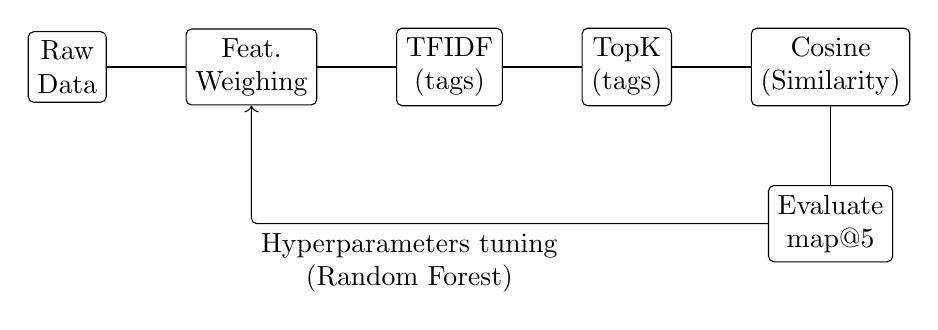
\begin{tikzpicture}[rounded corners=2pt]
\node [draw, align=center](rawdata) {Raw \\ Data};
\node [draw, align=center, right=of rawdata] (featweight) {Feat. \\ Weighing};
\node [draw,align=center, right=of featweight] (tfidf) {TFIDF \\ (tags)};
\node [draw,align=center, right=of tfidf] (topk) {TopK \\ (tags)};
\node [draw,align=center, right=of topk] (cos) {Cosine \\ (Similarity)};
\node [draw,align=center, below=of cos] (ev) {Evaluate \\ map@5};
\path[every node/.style={sloped,anchor=south,auto=false}]
 (rawdata) edge (featweight)
 (featweight) edge (tfidf)
 (tfidf) edge (topk)
 (topk) edge (cos)
 (cos) edge (ev);
 \draw[->] (ev) -| node[align=center, below right]{Hyperparameters tuning \\ (Random Forest)}  (featweight);
\end{tikzpicture}
   \end{center}
 \end{frame}
  \begin{frame}[standout]
  CSLIM BPR
  \end{frame}
  \begin{frame}{CSLIM BPR}
  \textbf{Preprocessing} \hfill \break
   Tag aggregation: 
  		\begin{itemize}
  		\item Select the topK most popular tags
  		\item For each tuple T of tags compute the logical AND
  		\item The result is a new feature, describing the items that share tags in T
  		\end{itemize}
  \end{frame}
	\begin{frame}{CSLIM BPR}
		\textbf{Our Improvements}
		\begin{itemize}
		\item \emph{Momentum} update rule implemented
		\item Samples to train the model are drawn from ICM and URM with different probabilities (in our case sampling more from ICM than URM gave better results).
		\end{itemize}
		\textbf{Results}  \hfill \break
		Even if this approach is a model-based one, we were able to achieve similar results with respect to the memory-based one:  \break \emph{ICM + URM Content Based}.
	\end{frame}
 	\begin{frame}{Training process}
   % diagram
   \begin{center}
   \begin{tikzpicture}[rounded corners=2pt]
\node [draw, align=center](rdata) {Raw \\ Data};
\node [draw, align=center, right=of rdata] (feataggr) {Feat. \\ Aggregation};
\node [draw,align=center, right=of feataggr] (bpr) {BPR-OPT};
\node [draw,align=center, right=of bpr] (model) {Model};
\path[every node/.style={sloped,anchor=south,auto=false}]
 (rawdata) edge (feataggr)
 (feataggr) edge (bpr);
\draw[->] (bpr) to [out=150,in=30,looseness=20, loop] node[align=center, above]{RMSPROP}  (bpr);
\draw[->] (bpr) edge (model);
\end{tikzpicture}
   \end{center}
 \end{frame}
 \begin{frame}[standout]
  Similarity Ensemble
  \end{frame}
  \begin{frame}{Similarity Ensemble}
  \textbf{Rationale}: 
  \begin{itemize}
  \item Combining different sets of features is very hard. Some features are more present than others and stating their relative importance is even harder
  \item Different models capture different aspects of the similarity between items
  \end{itemize}
  Our approach was to optimize each model separately and combine their similarity matrices.
  \end{frame}
  \begin{frame}{Similarity Ensemble}
  \metroset{block=fill}
  \begin{block}{The model}
  $$
  S_{ensemble} = \sum_{i \in M} \beta_i S_i
  $$
  \end{block}  
  Where M is the set of models. \break
  The coefficients $\beta_i$ are hyperparameters that we tune with Random Forest. \break
  \textbf{Properties}: 
  \begin{itemize}
  \item The similarity of each item with the others must be normalized
  \item For each item in $S_{ensemble}$  we keep only the topK similar items
  \item $S_{ensemble}$ is again normalized
  \end{itemize}
  \end{frame}
  \begin{frame}
   % diagram
   \begin{center}
   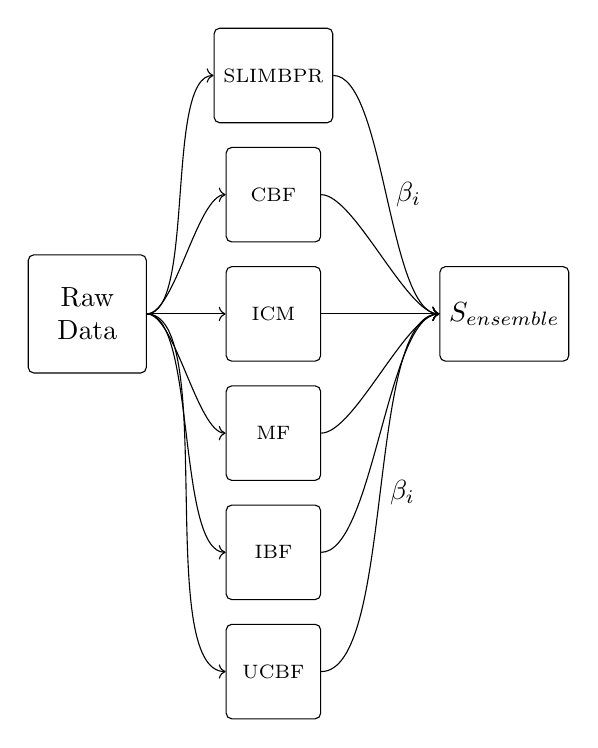
\begin{tikzpicture}[rounded corners=2pt]
\node [draw, align=center, minimum size=1.5cm](rdata) {Raw \\ Data};
\node [draw, align=center, right=of rdata, minimum size=1.2cm] (icm) {\scriptsize ICM};
\node [draw,align=center, above=0.3cm of icm, minimum size=1.2cm] (icmurm) { \scriptsize CBF};
\node [draw,align=center, above=0.3cm of icmurm, minimum size=1.2cm] (slimbpr) { \scriptsize SLIMBPR};
\node [draw,align=center, below=0.3cm of icm, minimum size=1.2cm] (mf) {\scriptsize MF};
\node [draw,align=center, below=0.3cm of mf, minimum size=1.2cm] (cf) {\scriptsize IBF};
\node [draw,align=center, below=0.3cm of cf, minimum size=1.2cm] (ucbf) {\scriptsize UCBF};
\node [draw,align=center, right=1.5cm of icm, minimum size=1.2cm] (s) { $S_{ensemble}$};
\draw[->] (rdata) to [out=0,in=180, looseness=0.5]  (ucbf);
\draw[->] (rdata) to [out=0,in=180, looseness=0.5]  (cf);
\draw[->] (rdata) to [out=0,in=180, looseness=0.5]  (icm);
\draw[->] (rdata) to [out=0,in=180, looseness=0.5]  (icmurm);
\draw[->] (rdata) to [out=0,in=180, looseness=0.5]  (slimbpr);
\draw[->] (rdata) to [out=0,in=180, looseness=0.5]  (mf);
% from nodes to S_ensemble
\draw[->] (ucbf) to [out=0,in=180, looseness=0.5]  node[align=center, right]{$\beta_i$} (s);
\draw[->] (cf) to [out=0,in=180, looseness=0.5]  (s);
\draw[->] (icm) to [out=0,in=180, looseness=0.5]  (s);
\draw[->] (icmurm) to [out=0,in=180, looseness=0.5]  (s);
\draw[->] (slimbpr) to [out=0,in=180, looseness=0.5]  node[align=center, right]{$\beta_i$}  (s);
\draw[->] (mf) to [out=0,in=180, looseness=0.5]  (s);
\end{tikzpicture}
   \end{center}
  \end{frame}
  \begin{frame}{Similarity Ensemble with Clustering}
  \begin{figure}
  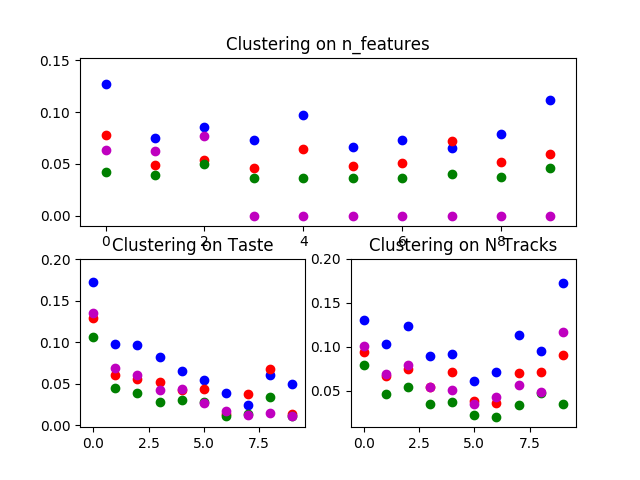
\includegraphics[width=0.8\linewidth]{cluster.png}
 \caption{This figure shows the performance of some models on users clustered with respect to different features.}
  \end{figure}
	
  \end{frame}
  \begin{frame}{Similarity Ensemble with Clustering}
   \metroset{block=fill}
  \begin{block}{The model}
  $$
  S_{ensemble_j} = \sum_{i \in M} \beta_{ij} S_i
  $$
  $$
  \hat{r}_i^{j}= r_i \cdot S_{ensemble_j} 
  $$
  \end{block}  
  Let $i$ be a user belonging to cluster $j$, the prediction $\hat{r}_i^{j}$ is computed from the ensemble similarity matrix personalized for that cluster ($S_{ensemble _j}$). 
  \end{frame}
  \section{Lessons Learned}
  \begin{frame}{Lessons Learned}
  \begin{itemize}
  \item Exploration/Exploitation trade off
  \item No Free Lunch theorem (No superior algorithm)
  \item Do Ensemble
  \end{itemize}
  
  \end{frame}
  \begin{frame}[standout]
  Thank you all!
  \end{frame}
\end{document}
